

\chapter{Predictive digital twins at scale for piles}
\label{DT}

This chapter develops a mathematical and computational foundation for digital twins of piles.

While the value proposition of digital twins has become widely appreciated, the technology itself remains in a custom production phase.



\section{State space model}




State space model, also called dynamic model, usually represents a class of directed probabilistic graphical model that describes the dependence between the hidden variables $\boldsymbol{Z} = (\boldsymbol{Z_0},\boldsymbol{Z_1},\boldsymbol{Z_2},...,\boldsymbol{Z_t})$ and the observed variables $\boldsymbol{X} = (\boldsymbol{X_1},\boldsymbol{X_2},...,\boldsymbol{X_t})$. This model also enables a dynamical updating for state estimation and control because they allow for recursive analysis of the systems in the time domain. As shown in \cref{fig: state-space-model}, this sequential updating feature is very suitable to geotechnical problems, because in our real life the observations typically appear in time series.



Based on the different assumptions for the model, state space model can be categorized as: Hidden Markov model, linear Gaussian state space model and Nonlinear non-Gaussian state space model.
\begin{figure}[H]
    \centering
    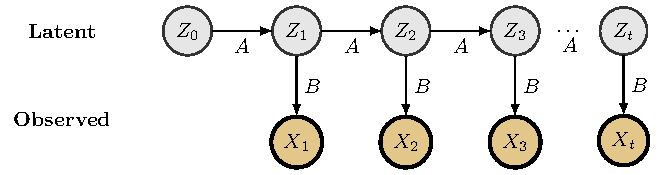
\includegraphics[width = 140mm]{Figures/figure-SSM.pdf}
    \caption{State space model}
    \label{fig: state-space-model}
\end{figure}
where gray circles $\boldsymbol{Z}$ are latent variable; bold outlines $\boldsymbol{X}$ are observed quantities; $A$ is the transition equation; $B$ is the observation equation. $A$ and $B$ are not time-varying.

\subsection{Hidden Markov model}

        
If the latent variables $\boldsymbol{Z} = (\boldsymbol{Z_0},\boldsymbol{Z_1},\boldsymbol{Z_2},...,\boldsymbol{Z_t})$ in \cref{fig:state-space-model} are discrete, we can treat the state space model as a hidden Markov model.  A hidden Markov model (HMM) allows us to talk about both observed events  $\boldsymbol{X}$ and hidden discrete events  $\boldsymbol{Z}$. A first-order hidden Markov model instantiates two simplifying assumptions as:

\begin{itemize}
      \item  First, as with a first-order Markov chain, the probability of a particular state depends
 only on the previous state:
         \begin{equation}
         P(Z_t|Z_0,Z_1,...,Z_{t-1})= P(Z_t|Z_{t-1})             
         \end{equation}      
      \item Second, the probability of an  observation $X_t$ depends only on the state that
 produced the observation $Z_t$ and not on any other states or any other observations:
          \begin{equation}
         P(Z_t|Z_0,Z_1,...,Z_{t-1})= P(Z_t|Z_{t-1})             
         \end{equation} 
\end{itemize}
In geotechnical area, filtering problem is more a quantity of interest. That is to say, given the current belief state $p(Z_{t-1}|X_{1:t-1})$, the primary concern next is how to calculate the belief state $p(Z_t|X_{1:t-1})$.
A prominent application for Hidden Markov model is addressing soil classification challenges with time series data. This is due to the discrete nature of the labeling predicament inherent in this context. However, the limitation for the HMM is also obvious. For the continuous state changing with time (e.g., soil stress, loading force or cumulative plastic strain), HMM is not suitable for such problem because infinite transition matrix $A$ does not exist. To solve this, we will discuss linear Gaussian model and nonlinear non-Gaussian model next. 







\subsection{Linear Gaussian state space model}

Linear Gaussian state space model is an exact Bayesian filtering solution, also called Kalman filter. Kalman filter describe a very specific setting, i.e., linear transition/observation equations and Gaussian noises. Since everything is Gaussian, we can perform the prediction and update steps in closed form,
 as we explain below:
% \setlength\abovedisplayskip{2pt}
% \setlength\belowdisplayskip{2pt}
\begin{equation}
\label{eq: Bayesian filtering}
\begin{aligned}
   & \boldsymbol{{z}_{t}}  =\boldsymbol{A} \boldsymbol{{z}_{t-1}}+\boldsymbol{w_{t}}  
  \ \ &\boldsymbol{w_{t}}   \sim \mathcal{N}\left(0, \boldsymbol{Q} \right) \\    
    &p(\boldsymbol{{z}_{t}}|\boldsymbol{{z}_{t-1}}) = \mathcal{N}(\boldsymbol{A} \boldsymbol{{z}_{t-1}},\boldsymbol{Q})    
    \\
     &\boldsymbol{{x}_{t}}=\boldsymbol{B} \boldsymbol{{z}_{t}}+\boldsymbol{v_{t}}  \ \ &\boldsymbol{v_{t}} \sim \mathcal{N}\left(0, \boldsymbol{R} \right)\\
     &p(\boldsymbol{{x}_{t}}|\boldsymbol{{z}_{t}}) = \mathcal{N}(\boldsymbol{B} \boldsymbol{{z}_{t}},\boldsymbol{R})   
\end{aligned}
\end{equation}
which stands for the prediction step and correction step, respectively.

The detailed principle of Kalman filter is not extensively emphasized here, because in geotechnical engineering, the transition and observation equations always show high nonlinearity. Once we add the SSM parameters to the state space model, the model is generally no longer linear Gaussian. Consequently
we must use some of the approximate online inference methods to be discussed below.

\subsection{Nonlinear non-Gaussian state space model}

Desipte the fact that some methods like Ensemble Kalman filter (EnKF), Unscented Kalman filter (UKF) or Extended kalman filter (EKF) can relax the linearity at some degree. These methods are still designed only for Gaussian posterior, which is not suitable for geotechnical problems with high nonlinearity. To handle the arbitrary posteriors, particle filtering which is based on Monte Carlo, can approximate the posterior with the increasing sampling points.



\section{Probabilistic graphical model: Control theory }




\section{Partially observable Markov decision process}

As shown in \cref{fig: POMDP}, based on Markov Chain, with introducing Rewards and Actions, it can form the basis of Partially observed Markov decision process.
\begin{figure}[H]
    \centering
    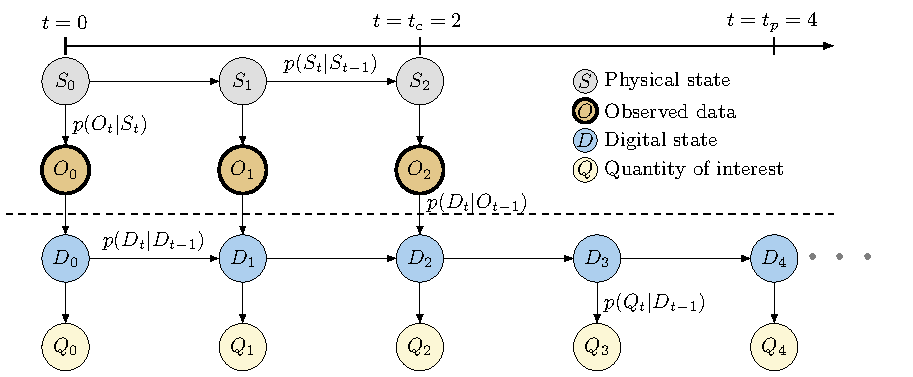
\includegraphics[width = 140mm]{Figures/figure-POMDP.pdf}
    \caption{Digital twin}
    \label{fig: POMDP}
\end{figure}
Generally, Digital Twin can be divided into two main parts, including (1) calibration and assimilation (2) Prediction, as shown in \cref{eq: DA_predict}  and \cref{eq: DA_assimilation}.
\begin{equation}
\begin{aligned}
& p(D_{0},...,D_{t_{c}},Q_{0},...,Q_{t_{c}},R_{0},...,R_{t_{c}}|o_{0},...,o_{t_{c}},u_{0},...,u_{t_{c}}) \\
& = \prod_{t=0}^{t_{c}}[\phi_{t}^{update}\phi_{t}^{QoI}\phi_{t}^{evaluation}] \label{eq: DA_predict}
\end{aligned}
\end{equation}
\begin{equation}
\begin{aligned}
    & p(D_{0},...,D_{t_{p}},Q_{0},...,Q_{t_{p}},R_{0},...,R_{t_{p}},U_{t_{c}+1},...,U_{t_{p}}|o_{0},...,o_{t_{c}},u_{0},...,u_{t_{c}}) \\
    & \propto \prod_{t=0}^{t_{p}}[\phi_{t}^{dynamics}\phi_{t}^{QoI}\phi_{t}^{evaluation}] \prod_{t=0}^{t_{c}}\phi_{t}^{assimilation} \prod_{t=t_{c}+1}^{t_{p}}\phi_{t}^{control} \label{eq: DA_assimilation}
\end{aligned}
\end{equation}
\section{Computational model-ICFEP}

\section{Planning and prediction via digital twin}